\section{mainwindow.h File Reference}
\label{mainwindow_8h}\index{mainwindow.h@{mainwindow.h}}
{\tt \#include $<$QDialog$>$}\par
{\tt \#include $<$QMain\-Window$>$}\par
{\tt \#include $<$QWidget$>$}\par
{\tt \#include $<$QText\-List\-Format$>$}\par
{\tt \#include $<$QText\-Block\-Format$>$}\par
{\tt \#include $<$Qt\-Xml$>$}\par
{\tt \#include $<$Qt\-Gui$>$}\par
{\tt \#include $<$QXml\-Simple\-Reader$>$}\par
{\tt \#include $<$QXml\-Input\-Source$>$}\par
{\tt \#include $<$QStandard\-Item\-Model$>$}\par
{\tt \#include $<$QAbstract\-Item\-Model$>$}\par
{\tt \#include $<$QAbstract\-List\-Model$>$}\par
{\tt \#include $<$QItem\-Selection\-Model$>$}\par
{\tt \#include $<$QAction$>$}\par
{\tt \#include $<$QApplication$>$}\par
{\tt \#include $<$QClipboard$>$}\par
{\tt \#include $<$QColor\-Dialog$>$}\par
{\tt \#include $<$QCombo\-Box$>$}\par
{\tt \#include $<$QFont\-Combo\-Box$>$}\par
{\tt \#include $<$QFile$>$}\par
{\tt \#include $<$QFile\-Dialog$>$}\par
{\tt \#include $<$QFile\-Info$>$}\par
{\tt \#include $<$QFont\-Database$>$}\par
{\tt \#include $<$QMenu$>$}\par
{\tt \#include $<$QMenu\-Bar$>$}\par
{\tt \#include $<$QPrint\-Dialog$>$}\par
{\tt \#include $<$QPrinter$>$}\par
{\tt \#include $<$QText\-Codec$>$}\par
{\tt \#include $<$QText\-Edit$>$}\par
{\tt \#include $<$QTool\-Bar$>$}\par
{\tt \#include $<$QText\-Cursor$>$}\par
{\tt \#include $<$QText\-List$>$}\par
{\tt \#include $<$Qt\-Debug$>$}\par
{\tt \#include $<$QClose\-Event$>$}\par
{\tt \#include $<$QMessage\-Box$>$}\par
{\tt \#include $<$QList$>$}\par
{\tt \#include $<$QHBox\-Layout$>$}\par
{\tt \#include $<$QSplitter$>$}\par
{\tt \#include $<$QSystem\-Tray\-Icon$>$}\par
{\tt \#include $<$QTree\-View$>$}\par
{\tt \#include $<$QList\-View$>$}\par
{\tt \#include $<$QStatus\-Bar$>$}\par
{\tt \#include \char`\"{}main.h\char`\"{}}\par
{\tt \#include \char`\"{}xmltree.h\char`\"{}}\par
{\tt \#include \char`\"{}treemodel.h\char`\"{}}\par
{\tt \#include \char`\"{}knowtreemodel.h\char`\"{}}\par
{\tt \#include \char`\"{}treescreen.h\char`\"{}}\par
{\tt \#include \char`\"{}editor.h\char`\"{}}\par
{\tt \#include \char`\"{}metaeditor.h\char`\"{}}\par
{\tt \#include \char`\"{}recordtablescreen.h\char`\"{}}\par
{\tt \#include \char`\"{}treeitem.h\char`\"{}}\par
{\tt \#include \char`\"{}appconfig.h\char`\"{}}\par
{\tt \#include \char`\"{}addnewrecord.h\char`\"{}}\par
{\tt \#include \char`\"{}editrecord.h\char`\"{}}\par
{\tt \#include \char`\"{}findscreen.h\char`\"{}}\par


Include dependency graph for mainwindow.h:\begin{figure}[H]
\begin{center}
\leavevmode
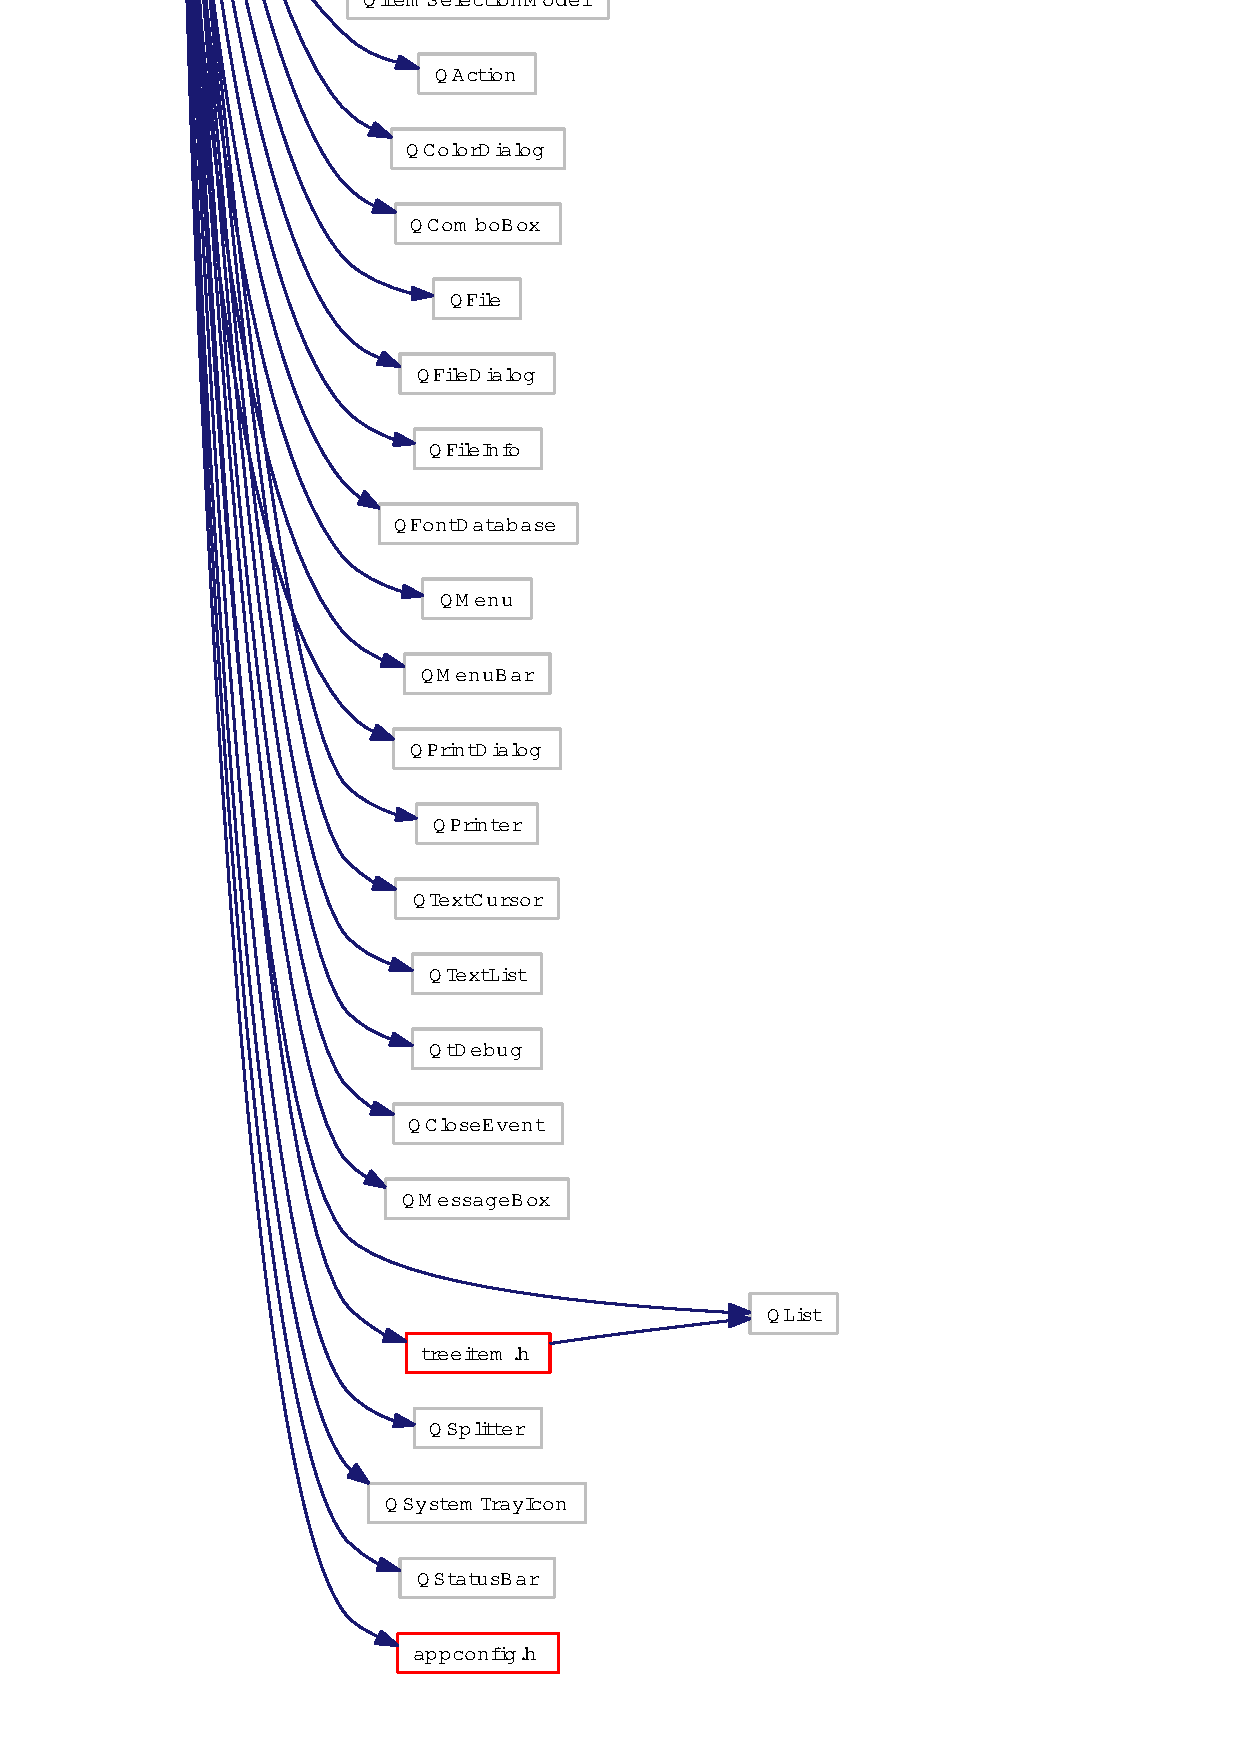
\includegraphics[width=366pt]{mainwindow_8h__incl}
\end{center}
\end{figure}


This graph shows which files directly or indirectly include this file:\begin{figure}[H]
\begin{center}
\leavevmode
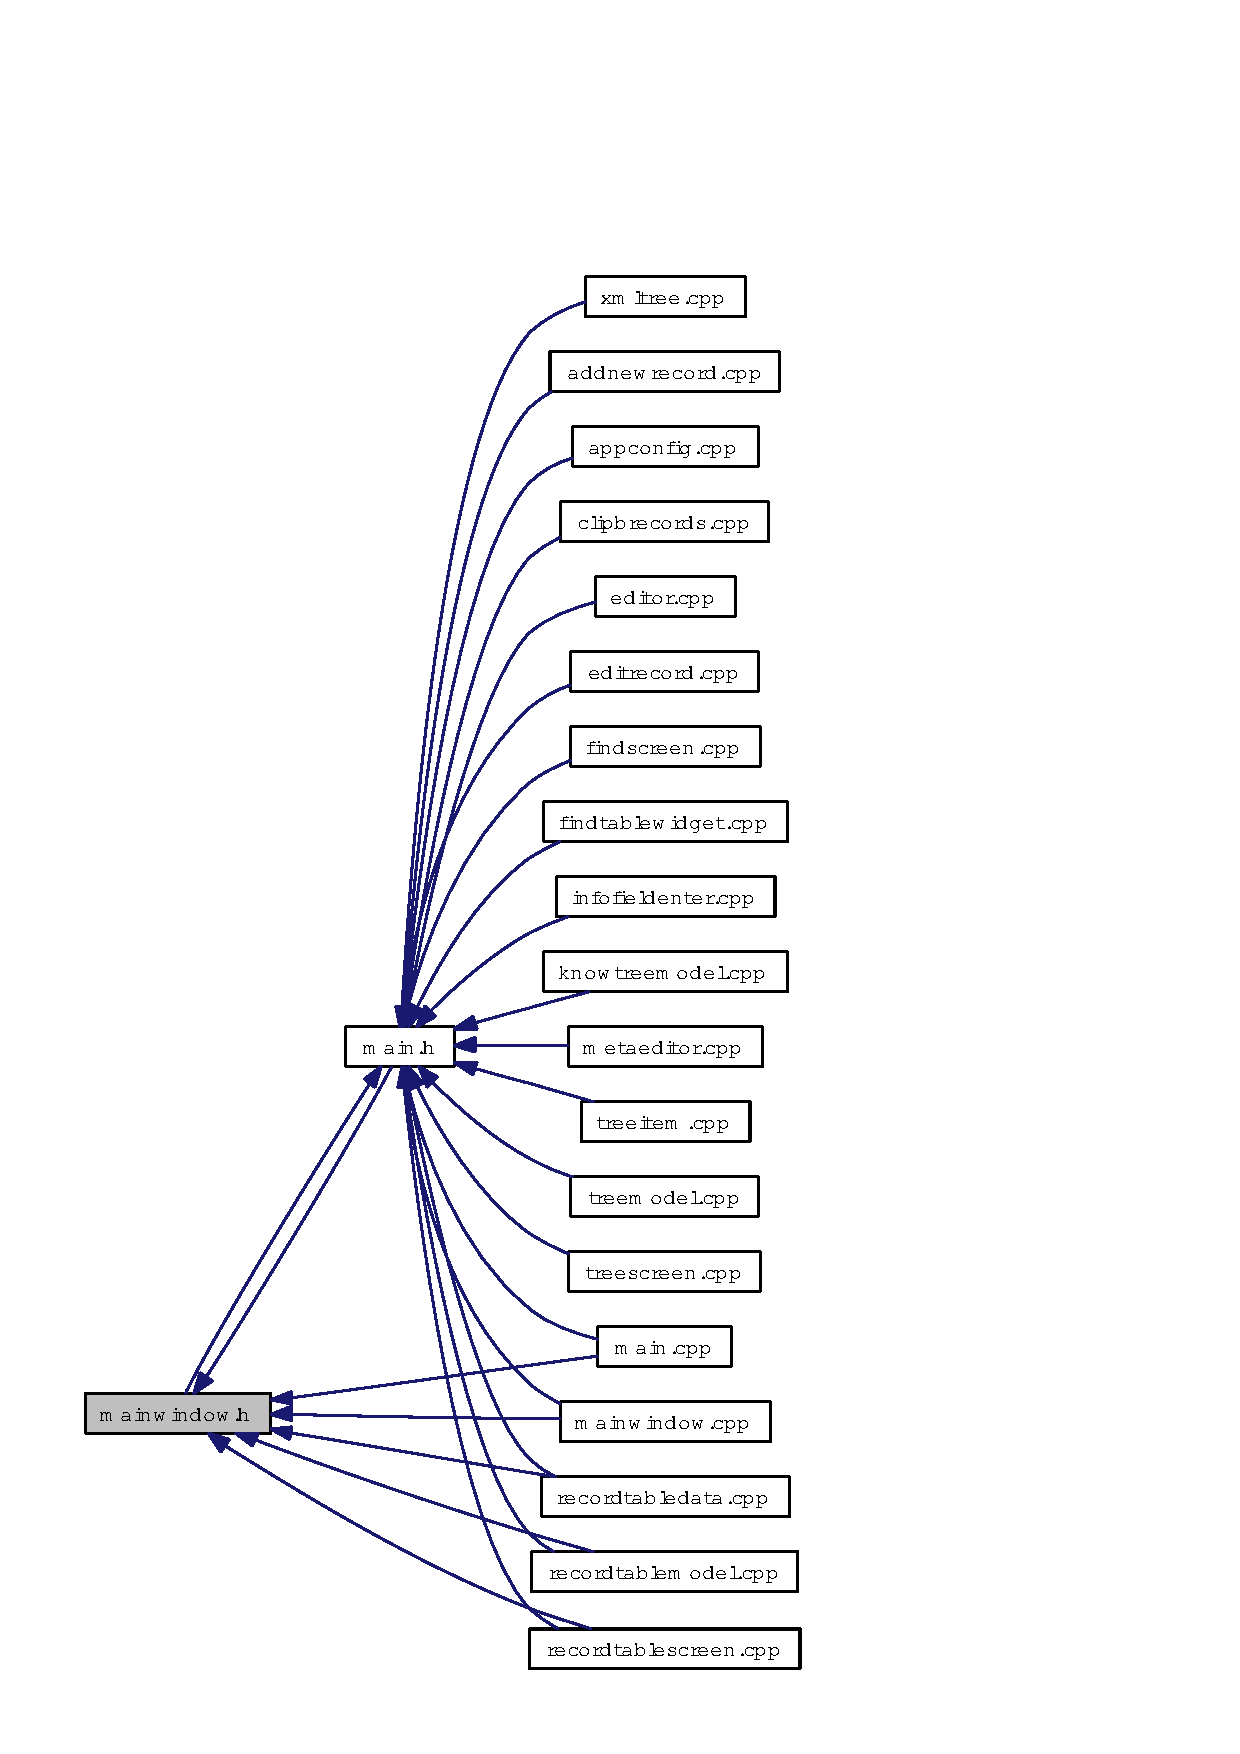
\includegraphics[width=194pt]{mainwindow_8h__dep__incl}
\end{center}
\end{figure}
\subsection*{Classes}
\begin{CompactItemize}
\item 
class {\bf mainwindow}
\end{CompactItemize}
\subsection*{Defines}
\begin{CompactItemize}
\item 
\#define {\bf ADD\_\-NEW\_\-RECORD\_\-TO\_\-END}~0
\item 
\#define {\bf ADD\_\-NEW\_\-RECORD\_\-BEFORE}~1
\item 
\#define {\bf ADD\_\-NEW\_\-RECORD\_\-AFTER}~2
\end{CompactItemize}


\subsection{Define Documentation}
\index{mainwindow.h@{mainwindow.h}!ADD_NEW_RECORD_AFTER@{ADD\_\-NEW\_\-RECORD\_\-AFTER}}
\index{ADD_NEW_RECORD_AFTER@{ADD\_\-NEW\_\-RECORD\_\-AFTER}!mainwindow.h@{mainwindow.h}}
\subsubsection{\setlength{\rightskip}{0pt plus 5cm}\#define ADD\_\-NEW\_\-RECORD\_\-AFTER~2}\label{mainwindow_8h_3850518597a1aac6ea8540bdb4dbc7ff}




Definition at line 68 of file mainwindow.h.

Referenced by recordtablescreen::add\_\-new\_\-after\_\-context(), and recordtabledata::insert\_\-new\_\-record().\index{mainwindow.h@{mainwindow.h}!ADD_NEW_RECORD_BEFORE@{ADD\_\-NEW\_\-RECORD\_\-BEFORE}}
\index{ADD_NEW_RECORD_BEFORE@{ADD\_\-NEW\_\-RECORD\_\-BEFORE}!mainwindow.h@{mainwindow.h}}
\subsubsection{\setlength{\rightskip}{0pt plus 5cm}\#define ADD\_\-NEW\_\-RECORD\_\-BEFORE~1}\label{mainwindow_8h_a265280e56bf1f4bf9309e95c12d0980}




Definition at line 67 of file mainwindow.h.

Referenced by recordtablescreen::add\_\-new\_\-before\_\-context(), and recordtabledata::insert\_\-new\_\-record().\index{mainwindow.h@{mainwindow.h}!ADD_NEW_RECORD_TO_END@{ADD\_\-NEW\_\-RECORD\_\-TO\_\-END}}
\index{ADD_NEW_RECORD_TO_END@{ADD\_\-NEW\_\-RECORD\_\-TO\_\-END}!mainwindow.h@{mainwindow.h}}
\subsubsection{\setlength{\rightskip}{0pt plus 5cm}\#define ADD\_\-NEW\_\-RECORD\_\-TO\_\-END~0}\label{mainwindow_8h_3ff28b5932200d5e6cac920029f0df0d}




Definition at line 66 of file mainwindow.h.

Referenced by recordtablescreen::add\_\-new\_\-toend\_\-context(), recordtabledata::insert\_\-new\_\-record(), and recordtablescreen::paste().